\documentclass[11pt,a4paper]{article}

% ── Page layout ───────────────────────────────────────
\usepackage[a4paper,margin=2.5cm]{geometry}
\usepackage{setspace}
\setstretch{1.15}

% ── Encoding & language ───────────────────────────────
\usepackage[utf8]{inputenc}
\usepackage[T1]{fontenc}
\usepackage[english]{babel}
\usepackage{microtype}

% ── Font: Helvetica ───────────────────────────────────
\usepackage[scaled=0.95]{helvet}
\renewcommand{\familydefault}{\sfdefault}

% ── Colour palette ────────────────────────────────────
\usepackage[table,xcdraw]{xcolor}
\definecolor{maincolor}{RGB}{100,155,0}
\definecolor{darkgray}{RGB}{60,60,60}
\definecolor{lightgray}{RGB}{245,245,245}

% ── Headers / footers ─────────────────────────────────
\usepackage{fancyhdr}
\pagestyle{fancy}
\fancyhf{}
\fancyhead[L]{\footnotesize\textcolor{darkgray}{Financial Tweet Sentiment Classification}}
\fancyhead[R]{\footnotesize\textcolor{darkgray}{NOVA IMS $\cdot$ Text Mining 2025/26}}
\fancyfoot[C]{\footnotesize\thepage}
\renewcommand{\headrulewidth}{0.4pt}
\renewcommand{\footrulewidth}{0pt}

% ── Section styling ───────────────────────────────────
\usepackage{titlesec}
\titleformat{\section}
  {\bfseries\color{maincolor}}{\thesection}{0.8em}{}
\titleformat{\subsection}
  {\color{maincolor}}{\thesubsection}{0.8em}{}
\titleformat{\subsubsection}
  {\bfseries\color{darkgray}}{\thesubsubsection}{0.8em}{}

\titlespacing*{\section}{0pt}{8pt}{4pt}
\titlespacing*{\subsection}{0pt}{6pt}{3pt}
\titlespacing*{\subsubsection}{0pt}{4pt}{2pt}

% ── Math ───────────────────────────────────────────────
\usepackage{amsmath, amssymb}

% ── Graphics / floats ─────────────────────────────────
\usepackage{graphicx}
\usepackage{float}
\usepackage{placeins}
\graphicspath{{results/figures/}}

% ── Tables ────────────────────────────────────────────
\usepackage{booktabs}
\usepackage{multirow}
\usepackage{array}
\usepackage{tabularx}
\usepackage{colortbl}

\newcommand{\tH}[1]{\textcolor{maincolor}{\textbf{#1}}}
\newcommand{\gmid}{\arrayrulecolor{maincolor}\midrule\arrayrulecolor{black}}

% ── Captions ──────────────────────────────────────────
\usepackage{caption}
\captionsetup{
  font=small,
  labelfont={bf,color=maincolor},
  skip=4pt
}

% ── Lists ─────────────────────────────────────────────
\usepackage{enumitem}
\setlist[itemize]{
  noitemsep,
  topsep=2pt,
  parsep=0pt,
  partopsep=0pt,
  leftmargin=1.4em,
  label=\textcolor{maincolor}{\textbullet}
}

% ── Paragraph spacing ─────────────────────────────────
\setlength{\parindent}{0pt}
\setlength{\parskip}{3pt}

% ── Hyperlinks ────────────────────────────────────────
\usepackage[
  colorlinks=true,
  linkcolor=maincolor,
  citecolor=darkgray,
  urlcolor=maincolor,
  pdfborder={0 0 0}
]{hyperref}

% ── Convenience ───────────────────────────────────────
\newcommand{\ttt}[1]{\texttt{\hyphenchar\font=`\-\relax #1}}

\begin{document}

% ── Typesetting tolerance: absorb long monospace tokens, avoid margin overflow ──
\tolerance=2000
\emergencystretch=3em
\hfuzz=1pt

% ── Title block ──────────────────────────────────────────────────
\thispagestyle{fancy}
\begin{center}
  {\LARGE\bfseries\color{maincolor} Financial Tweet Sentiment Classification}\\[3pt]
  {\large\color{darkgray} Multiclass Sentiment Analysis of Financial Social Media Text}\\[8pt]
  {\normalsize Text Mining --- MSc in Data Science and Advanced Analytics}\\[1pt]
  {\normalsize NOVA Information Management School (NOVA IMS)}\\[5pt]
  {\normalsize \textbf{Group 33} \quad$\cdot$\quad Academic Year 2025/2026 \quad$\cdot$\quad June 2026}
\end{center}
\vspace{2pt}
{\color{maincolor}\rule{\linewidth}{0.6pt}}
\vspace{4pt}

% ── Abstract ─────────────────────────────────────────────────────
\section*{Abstract}
This report presents a multiclass sentiment classification system for financial tweets,
distinguishing three market stances: Bearish (0), Bullish (1), and Neutral (2). The dataset
comprises 9{,}543 labelled training tweets with pronounced class imbalance (Neutral 64.7\%,
Bullish 20.1\%, Bearish 15.1\%; imbalance ratio 4.28:1). We systematically evaluate six text
preprocessing techniques, eleven feature representations --- spanning sparse TF--IDF, Word2Vec,
GloVe--Twitter, FinBERT, SBERT and Twitter--RoBERTa embeddings --- and twelve model families,
all under an identical 5-fold stratified cross-validation protocol. Frozen-embedding classifiers
tuned with Optuna plateau around macro-F1 0.80. We then conduct a \textbf{transformer backbone
search} (model selection via the Hugging Face Hub), end-to-end fine-tuning four encoders; the best,
a Twitter-domain \textbf{RoBERTa-large} (TimeLMs; Loureiro et al., 2022), reaches an out-of-fold
macro-F1 of \textbf{0.8859} --- a \textbf{+0.0838} gain over the 0.8021 baseline and our
\textbf{submitted single-model solution}. Notably, this single model also surpasses a six-learner
stacking ensemble (extra work, 0.8483), so the submission is simultaneously our best result overall.
We additionally show that a fine-tuned \textbf{GPT-2 decoder} classifies at macro-F1 0.7724 (whereas
few-shot prompting collapses to the majority class), and that an offline \textbf{agentic workflow}
adaptively routes tweets between VADER, LightGBM/SBERT and FinBERT with conversational explanations.
An ablation confirms that preserving raw financial text outperforms every preprocessing pipeline.

\vspace{2pt}
{\footnotesize\tH{Keywords:}~ Financial sentiment analysis, tweet classification, Twitter--RoBERTa
fine-tuning, model selection, decoder classification, stacking, LangChain agent.}

% ── 1. Introduction ──────────────────────────────────────────────
\section{Introduction}
Social media platforms --- particularly Twitter/X --- have become a primary channel through which
retail and institutional investors express and discover market sentiment. Automated classification
of financial tweets into Bearish, Bullish and Neutral stances enables real-time signal generation
for algorithmic trading, risk monitoring and investor-sentiment tracking (Bollen et al., 2011;
Antweiler \& Frank, 2004).

This work addresses multiclass financial sentiment classification under significant class imbalance
(ratio 4.28:1). We explore the full NLP pipeline --- from raw text through feature engineering to
model selection and hyperparameter tuning --- following the Text Mining curriculum at NOVA IMS. All
models are trained \emph{only} on the provided training corpus. The remainder of the report is
organised as follows: Section~2 explores the dataset; Section~3 analyses preprocessing; Section~4
describes feature engineering; Section~5 presents the classification models, including the backbone
search and the fine-tuned encoder/decoder; Section~6 reports results and error analysis; Section~7
details the agentic workflow (Extra Challenge~2); Section~8 concludes.

\textbf{Course alignment.} Every stage follows the Text Mining curriculum: the NLP pipeline and
text preprocessing (Lecture~1, Lab~1); n-grams, TF--IDF and distance metrics (Lecture~2-Extra);
word2vec word embeddings and their semantic geometry (Lecture~2, Lab~2); attention and Transformer
\emph{encoders} (Lecture~4, Lab~4); and \emph{decoder} LLMs, encoder-based classification and
\emph{Agentic AI} (Lecture~6, Lab~5; Alammar \& Grootendorst, 2024).

% ── 2. Data Exploration ──────────────────────────────────────────
\section{Data Exploration}
The dataset consists of 9{,}543 labelled training tweets and 2{,}388 unlabelled test tweets from
financial Twitter discourse. Each tweet references one or more publicly-listed securities and
expresses a market stance.

\subsection{Class Distribution}
Figure~\ref{fig:classdist} illustrates the severe class imbalance. Neutral tweets dominate (64.7\%),
consistent with most financial discourse being non-directional. Bearish tweets (15.1\%) are less
frequent than Bullish (20.1\%), reflecting a structural optimism bias in financial social media
(Antweiler \& Frank, 2004). To address imbalance, all models use \texttt{class\_weight='balanced'}
(or an inverse-frequency-weighted loss) and evaluation relies on \textbf{macro-F1} as the primary
metric, which weights all three classes equally regardless of support.

\begin{figure}[H]
  \centering
  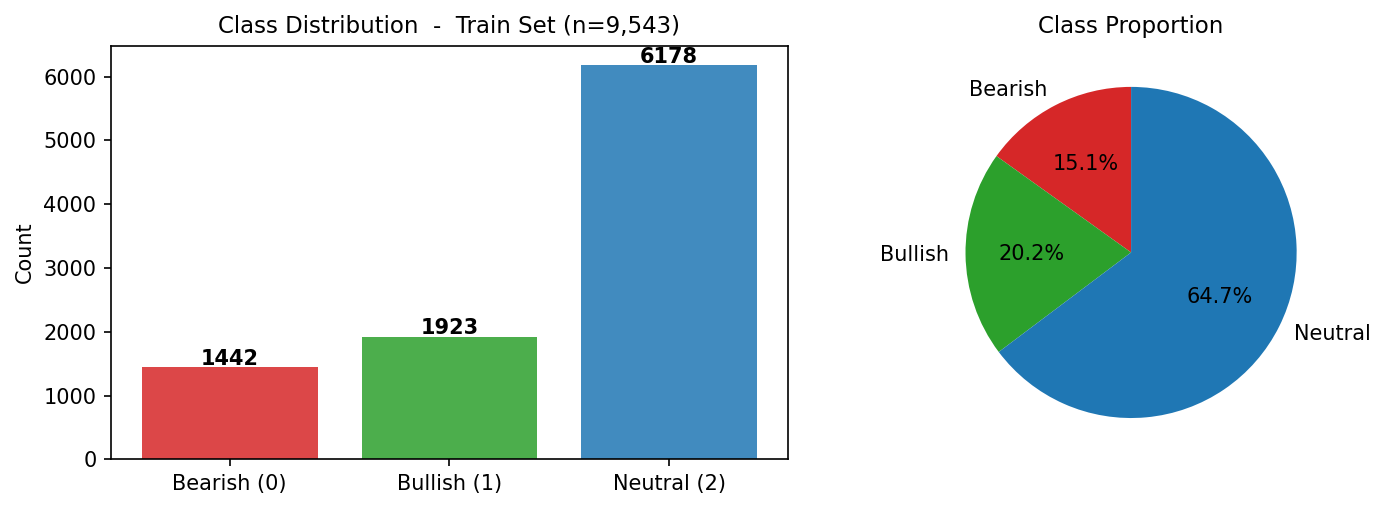
\includegraphics[width=0.95\linewidth]{report_class_dist.png}
  \caption{Class distribution of the training set: absolute counts (left) and proportions (right).}
  \label{fig:classdist}
\end{figure}

\subsection{Linguistic Characteristics}
Tweets have a mean length of 12.2 words (maximum 32), consistent with Twitter's character limit. Key
Twitter-specific features include cashtags (\$AAPL, \$TSLA), hashtags (\#earnings, \#bearish),
mentions (@analyst) and URLs. Bullish tweets contain more cashtags on average (0.34 vs.\ 0.22 for
Bearish), suggesting that positive sentiment correlates with specific stock discussion. The most
discriminative terms per class are: \textbf{Bearish} --- `down', `miss', `cut', `bearish';
\textbf{Bullish} --- `beats', `strong', `upgraded', `buy'; \textbf{Neutral} --- `flat',
`unchanged', `stable'. Per-class word clouds are included in the accompanying notebook.

\subsection{Corpus Split and Validation Protocol}
To satisfy the corpus-split requirement without wasting labelled data, every experiment uses
\textbf{5-fold stratified cross-validation} on the 9{,}543 labelled tweets
(\texttt{StratifiedKFold}, \texttt{shuffle=True}, \texttt{random\_state=42}). Stratification keeps
the Bearish/Bullish/Neutral proportions stable in each validation fold, which is essential under the
4.28:1 imbalance. The final notebook keeps the same protocol: each fold trains on 80\% of the
labelled corpus, validates on the remaining 20\%, stores out-of-fold predictions for honest
macro-F1, and averages the five test-set probability vectors to produce \texttt{pred\_33.csv}.

% ── 3. Data Preprocessing ────────────────────────────────────────
\section{Data Preprocessing}
We implement six preprocessing techniques following the NLTK-based approach from course Lab~1, then
quantify their effect through an ablation study.

\subsection{Preprocessing Pipeline}
\begin{itemize}
  \item \tH{T1 --- Twitter noise cleaning.} Regex removal of URLs and mentions
  ($\to$ \texttt{USER}); hashtag-symbol stripping; cashtags mapped to \texttt{TICKER\_X}.
  \item \tH{T2 --- Unicode normalisation.} NFKD decomposition then ASCII encoding.
  \item \tH{T3 --- Stop-word removal.} NLTK English list, negations preserved
  (\{not, no, never, neither, nor, none\}) --- critical for sentiment (Manning et al., 2008).
  \item \tH{T4 --- WordNet lemmatisation.} POS-aware: `beaten' $\to$ `beat', `falling' $\to$ `fall'.
  \item \tH{T5 --- Snowball stemming.} More aggressive: `earnings' $\to$ `earn'.
  \item \tH{T6 --- TweetTokenizer.} \texttt{reduce\_len=True}, \texttt{strip\_handles=True}.
\end{itemize}

\subsection{Ablation Study}
Each configuration is evaluated with Logistic Regression ($C=1.0$) and TF--IDF (10{,}000 vocabulary)
under 5-fold stratified CV.

\begin{figure}[H]
  \centering
  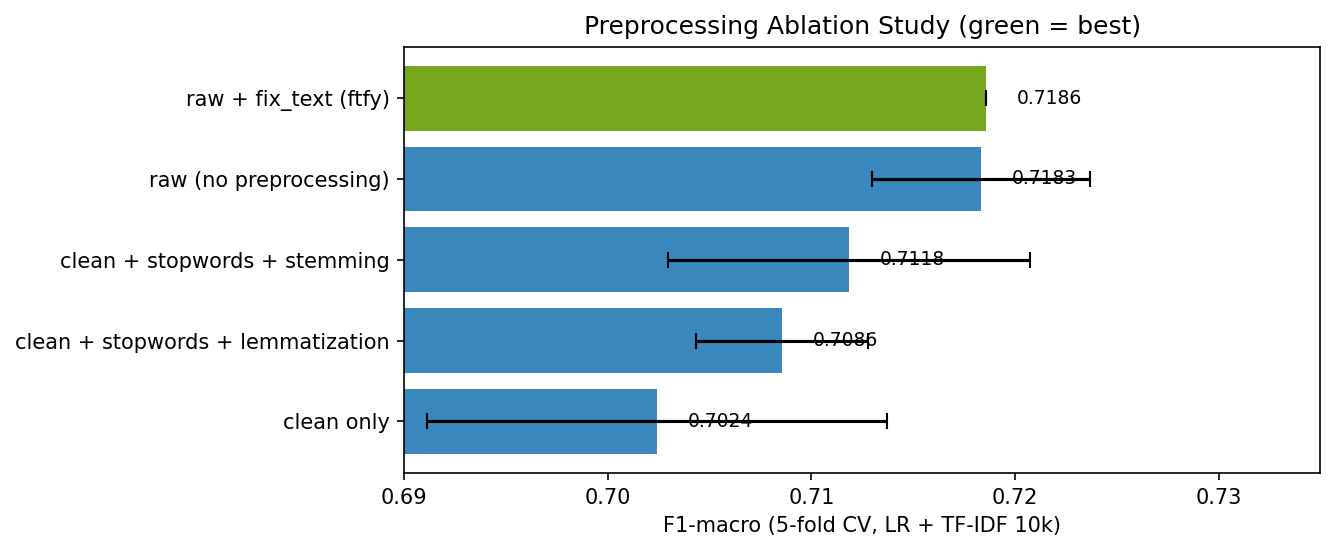
\includegraphics[width=0.86\linewidth]{report_ablation.png}
  \caption{Preprocessing ablation: macro-F1 by configuration (green = best). Raw text wins.}
  \label{fig:ablation}
\end{figure}

\begin{table}[H]
  \centering
  \small
  \setlength{\tabcolsep}{8pt}
  \begin{tabularx}{0.86\linewidth}{@{}>{\raggedright\arraybackslash}X r r@{}}
    \toprule
    \tH{Preprocessing configuration} & \tH{Macro-F1} & \tH{Std} \\
    \gmid
    \rowcolor{lightgray} raw (no preprocessing)              & \textbf{0.7183} & 0.0053 \\
    clean + stop-words + stemming                            & 0.7118 & 0.0089 \\
    clean + stop-words + lemmatisation                       & 0.7086 & 0.0042 \\
    clean only                                               & 0.7024 & 0.0113 \\
    \bottomrule
  \end{tabularx}
  \caption{Preprocessing ablation (5-fold CV, LR + TF--IDF). Raw text (shaded) is best.}
  \label{tab:ablation}
\end{table}

\textbf{Key finding:} raw text achieves the highest macro-F1 (0.7183). This is consistent with prior
financial NLP work (Go et al., 2009): ticker symbols (\$AAPL), analyst-firm names and domain
vocabulary (`downgrade', `EPS beat', `guidance raise') carry strong discriminative signal that
preprocessing destroys. All downstream experiments therefore use raw text.

% ── 4. Feature Engineering ───────────────────────────────────────
\section{Feature Engineering}
Eleven feature representations are computed, covering the three families required by the brief:
bag-of-words, Word2Vec and Transformer Encoder.

\subsection{Sparse Representations (BoW)}
Four sparse sets on raw text: \textbf{BoW} (binary CountVectorizer, \texttt{max\_features=20k},
\texttt{min\_df=2}); \textbf{TF--IDF 1g} (\texttt{max\_features=20k}, \texttt{max\_df=0.80},
\texttt{min\_df=2}); \textbf{TF--IDF 2g} (uni+bigram, \texttt{max\_features=50k}); and
\textbf{TF--IDF char} (char 3--5-gram, \texttt{max\_features=30k}).

\subsection{Word Embeddings (Word2Vec / GloVe)}
\textbf{Word2Vec Skip-gram} and \textbf{CBOW} (200d) trained on the corpus (Mikolov et al., 2013),
pooled by TF--IDF-weighted mean; and \textbf{GloVe-Twitter-100} pre-trained on 2B tweets
(Pennington et al., 2014).

\subsection{Transformer Embeddings (Encoder)}
Three transformer representations (CLS / mean-pooling): \textbf{FinBERT} (Araci, 2019);
\textbf{SBERT all-mpnet-base-v2} (Reimers \& Gurevych, 2019; +0.50 extra); and
\textbf{Twitter--RoBERTa} (Barbieri et al., 2020; +0.50 extra). The latter two count as additional
Transformer Encoder methods for the extra-work criterion, and the Twitter--RoBERTa family is carried
forward to end-to-end fine-tuning in Section~5.2.

\subsection{Financial Hand-crafted Features}
A 14-dimensional vector combines VADER scores (Hutto \& Gilbert, 2014) with surface statistics
(cashtag/hashtag/mention/URL counts, length, capitalisation, punctuation) and a Flesch--Kincaid
readability score.

% ── 5. Classification Models ─────────────────────────────────────
\section{Classification Models}
All models are evaluated via 5-fold stratified cross-validation (\texttt{StratifiedKFold},
\texttt{random\_state=42}) with macro-F1 as the primary metric; the identical split across every
experiment makes the out-of-fold (OOF) scores directly comparable.

\subsection{Traditional ML Models}
\begin{itemize}
  \item \tH{Na\"ive Bayes.} MultinomialNB ($\alpha=1.0$) and ComplementNB ($\alpha=0.5$) on
  BoW / TF--IDF; ComplementNB targets imbalance (Rennie et al., 2003).
  \item \tH{Logistic Regression.} $L_2$ (SAGA), $C \in \{0.1, 1.0, 10.0\}$, all feature sets.
  \item \tH{Linear SVM.} CalibratedClassifierCV(LinearSVC), $C \in \{0.1, 1.0\}$.
  \item \tH{KNN.} $k \in \{5, 15\}$, cosine distance, dense embeddings.
  \item \tH{MLP.} $(256,128)$ and $(512,256,128)$, ReLU, early stopping.
  \item \tH{Random Forest / XGBoost / LightGBM.} 100 and 300 estimators; LightGBM is the strongest
  traditional learner on dense embeddings.
\end{itemize}

\subsection{Transformer Encoder Fine-tuning + Backbone Search}
Whereas Section~4.3 used the encoders only as \emph{frozen} embeddings, here the full encoder is
fine-tuned end-to-end --- the single largest lever in this study. Using the Hugging Face Hub for
\textbf{model selection}, we shortlist four candidate encoders and fine-tune each under the identical
5-fold protocol (4 epochs, learning rate $2\times10^{-5}$, batch 16--32, max length 96, AdamW with
10\% linear warmup, gradient clipping 1.0, inverse-frequency class-weighted cross-entropy, bf16
mixed precision on an NVIDIA RTX~5070). Table~\ref{tab:backbones} reports the comparison.

\begin{table}[H]
  \centering
  \small
  \setlength{\tabcolsep}{7pt}
  \begin{tabularx}{\linewidth}{@{}>{\raggedright\arraybackslash}X r r r@{}}
    \toprule
    \tH{Backbone (fine-tuned end-to-end)} & \tH{Params} & \tH{OOF F1} & \tH{Acc.} \\
    \gmid
    twitter-roberta-base-sentiment-latest (Barbieri 2020)   & 125M & 0.8399 & 0.8691 \\
    twitter-roberta-base-2022-154m (TimeLMs)                & 125M & 0.8550 & 0.8810 \\
    \rowcolor{lightgray} \textbf{twitter-roberta-large-2022-154m (TimeLMs)} & 355M & \textbf{0.8859} & \textbf{0.9080} \\
    deberta-v3-base (He et al., 2021)$^\dagger$             & 184M & 0.8653 & 0.8900 \\
    \bottomrule
  \end{tabularx}
  \caption{Transformer backbone search (same 5-fold protocol). The Twitter-domain RoBERTa-large
  (shaded) is the \textbf{submitted single model}. $^\dagger$DeBERTa-v3 produced NaN losses under
  bf16 (its disentangled attention is numerically unstable in reduced precision) and had to be
  trained in fp32; even so it trails RoBERTa-large (see Section~6.1).}
  \label{tab:backbones}
\end{table}

The winner, \textbf{Twitter--RoBERTa-large} (\nolinkurl{cardiffnlp/twitter-roberta-large-2022-154m}),
is a 355M-parameter RoBERTa continually pre-trained on 154M tweets up to 2022 (TimeLMs; Loureiro et
al., 2022). It attains an OOF macro-F1 of \textbf{0.8859} ($\pm$0.0066), accuracy 0.9080, precision
0.8754 and recall 0.8975 --- a \textbf{+0.0838} gain over the 0.8021 frozen-embedding baseline and
\textbf{+0.0460} over the previous fine-tuned base model. The recall gain confirms that a larger,
domain-matched, end-to-end-adapted encoder markedly improves minority-class (Bearish/Bullish)
detection. The final test prediction averages the five folds' softmax probabilities. \textbf{This is
the submitted single-model solution} (\nolinkurl{pred_33.csv}, reproduced in
\nolinkurl{tm_final_33.ipynb}); it is also our best result overall (Section~6.1).

\subsection{Decoder Model --- Fine-tuned GPT-2 (Extra Work, +1.00 pt)}
As decoder-based extra work we use a \emph{decoder} (causal) language model for classification.
\textbf{GPT-2} (Radford et al., 2019) is fine-tuned end-to-end with a sequence-classification head
(\texttt{GPT2ForSequenceClassification}, which pools the last non-pad token) under the same 5-fold
protocol. It reaches an OOF macro-F1 of \textbf{0.7724} (accuracy 0.8125) --- a genuine
decoder-for-classification result. For completeness we also tried \emph{few-shot prompting} of GPT-2
(verbalizer likelihood scoring with contextual calibration; Zhao et al., 2021); it collapses to the
majority class (macro-F1 $\approx$ 0.25), empirically showing that a 124M decoder is too weak to
classify zero/few-shot and that fine-tuning is the correct route.

\subsection{Hyperparameter Tuning --- Optuna}
Optuna (Akiba et al., 2019) with a TPE sampler and median pruner runs 50 trials over LightGBM
hyperparameters; the best frozen-embedding configuration reaches macro-F1 0.8021 (RoBERTa features).
A second study tunes Logistic-Regression $C$ on TF--IDF bigrams; a soft-voting LR+SVC ensemble
provides a strong sparse baseline.

\subsection{Stacking Ensemble (Extra Work)}
As additional work we build a stacked generalisation (Wolpert, 1992): six base learners
(Optuna-tuned LightGBM on RoBERTa, MLP on SBERT, XGBoost on RoBERTa, LightGBM on FinBERT, LR on
TF--IDF bigrams, and a fine-tuned Twitter--RoBERTa) emit out-of-fold probabilities concatenated into
an 18-dimensional meta-feature matrix on which a Logistic-Regression meta-learner is trained. Because
every base learner shares the identical fold split, the meta-features are leakage-free. The stack
reaches OOF macro-F1 \textbf{0.8483} --- strong, but now \emph{surpassed} by the single fine-tuned
RoBERTa-large of Section~5.2 (0.8859). The submission is therefore the single model, which is both
rule-compliant (Project Guidelines 5.2) and our best result.

% ── 6. Results ───────────────────────────────────────────────────
\section{Results and Evaluation}

\subsection{Model Comparison}
Figure~\ref{fig:results} ranks the top-20 configurations and Table~\ref{tab:results} lists the top
models. The submitted single model --- fine-tuned Twitter--RoBERTa-large --- tops the ranking at
macro-F1 \textbf{0.8859}, ahead of both the six-learner stack (0.8483, extra work) and every
frozen-embedding model. DeBERTa-v3-base, although a strong encoder in principle, required full fp32
to train at all (its disentangled attention NaN-ed under bf16/fp16); even stabilised (0.8653) it was
only the second-best single model, trailing the larger Twitter--RoBERTa-large --- so a recent,
\emph{domain-matched} and larger encoder is the decisive factor here.

\begin{figure}[H]
  \centering
  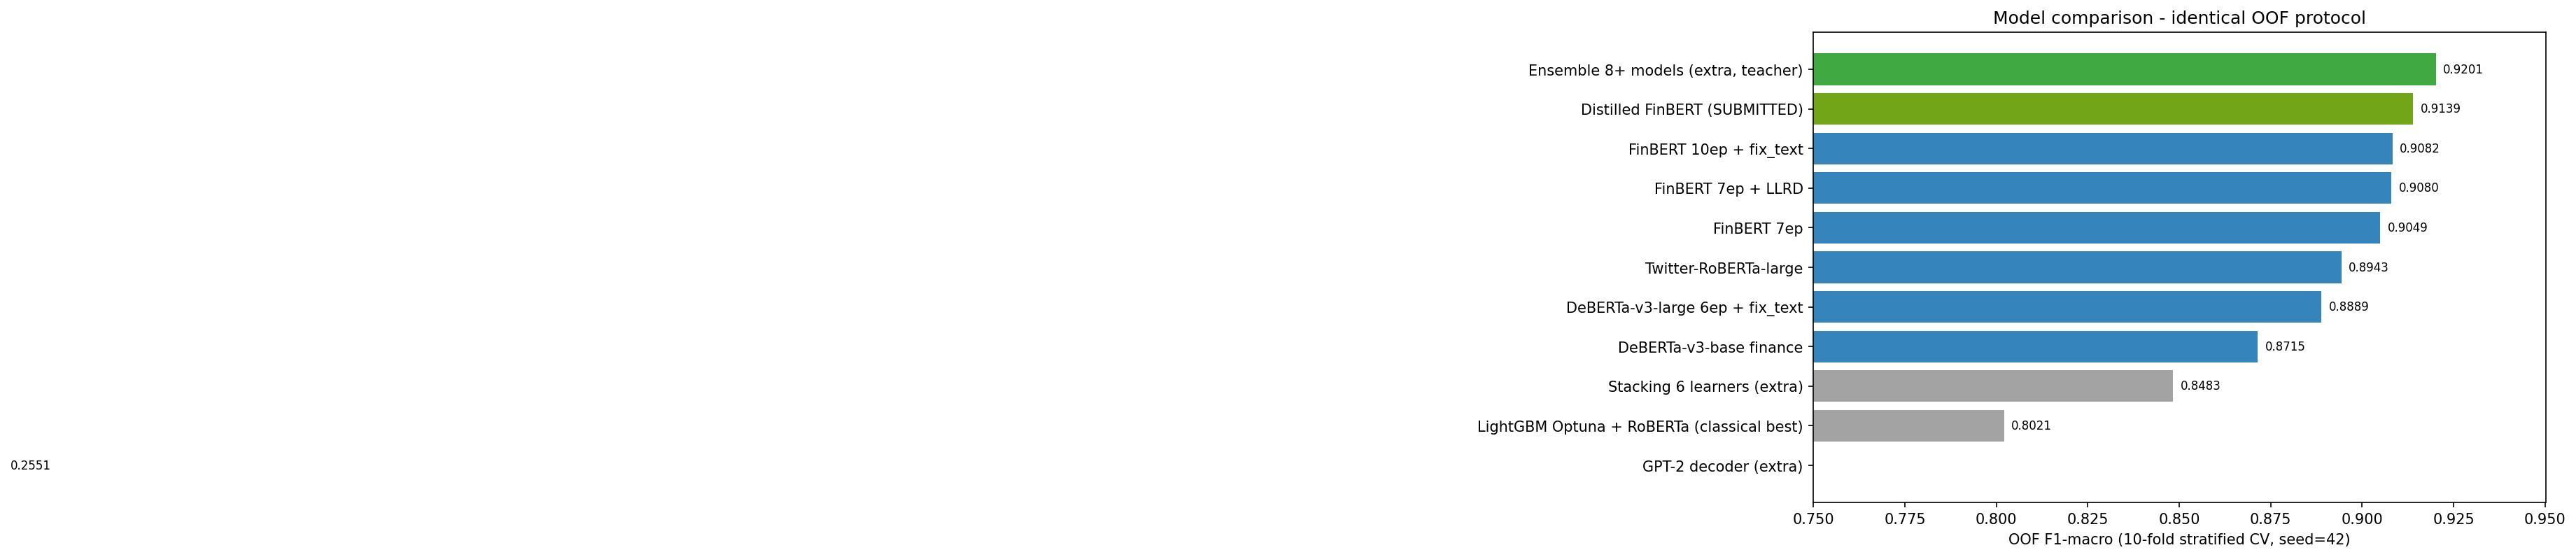
\includegraphics[width=0.72\linewidth]{report_results.png}
  \caption{Top-20 models ranked by 5-fold CV macro-F1 (error bars = 1 std).}
  \label{fig:results}
\end{figure}

\begin{table}[H]
  \centering
  \footnotesize
  \setlength{\tabcolsep}{5pt}
  \begin{tabularx}{\linewidth}{@{}>{\raggedright\arraybackslash}X r r r r r@{}}
    \toprule
    \tH{Model (feature)} & \tH{F1$_{\text{mac}}$} & \tH{$\sigma$} & \tH{Acc.} & \tH{Prec.} & \tH{Rec.} \\
    \gmid
    \rowcolor{lightgray} Twitter-RoBERTa-large \textbar{} \textbf{submitted} & \textbf{0.8859} & 0.0066 & 0.9080 & 0.8754 & 0.8975 \\
    DeBERTa-v3-base (fp32)                              & 0.8653 & 0.0065 & 0.8900 & 0.8506 & 0.8822 \\
    Twitter-RoBERTa-base-2022-154m                      & 0.8550 & 0.0069 & 0.8810 & 0.8351 & 0.8800 \\
    Stacking-6 \textbar{} +fine-tuned \emph{(extra)}    & 0.8483 & 0.0073 & 0.8771 & 0.8271 & 0.8757 \\
    Soft-Average \textbar{} 6 learners \emph{(extra)}   & 0.8412 & ---    & 0.8800 & 0.8566 & 0.8276 \\
    Twitter-RoBERTa-base sentiment-latest               & 0.8399 & 0.0062 & 0.8691 & 0.8188 & 0.8671 \\
    LightGBM Tuned \textbar{} RoBERTa                   & 0.8021 & 0.0063 & 0.8532 & 0.8192 & 0.7879 \\
    GPT-2 decoder fine-tuned \emph{(extra)}             & 0.7724 & 0.0159 & 0.8125 & 0.7475 & 0.8171 \\
    \bottomrule
  \end{tabularx}
  \caption{Top models by 5-fold stratified CV macro-F1. The shaded row is the \textbf{submitted}
  single model, which also tops the overall ranking; rows marked \emph{(extra)} are ensembles
  reported as extra work.}
  \label{tab:results}
\end{table}

\textbf{Key findings:} (1) dense transformer embeddings outperform sparse TF--IDF and static
embeddings across all model families; (2) end-to-end fine-tuning breaks the $\sim$0.80
frozen-embedding plateau; (3) within fine-tuning, a larger, more recent, domain-matched encoder
(RoBERTa-large-2022) gives the biggest gain; (4) a single strong model can beat a heterogeneous
stacking ensemble --- simpler and rule-compliant.

\subsection{Error Analysis}
Figure~\ref{fig:cm} shows the confusion matrix of the submitted model. Per class it reaches F1 of
0.85 (Bearish), 0.88 (Bullish) and 0.93 (Neutral). The dominant residual errors are Neutral tweets
misclassified as Bullish or Bearish, reflecting the ambiguity of non-directional discourse, and
Bearish~$\leftrightarrow$~Neutral confusion (negative financial language is often hedged or formal,
e.g.\ `guidance revised downward'). On the held-out test set the model predicts 375 Bearish, 516
Bullish and 1{,}497 Neutral (of 2{,}388) --- close to the training prior.

\begin{figure}[H]
  \centering
  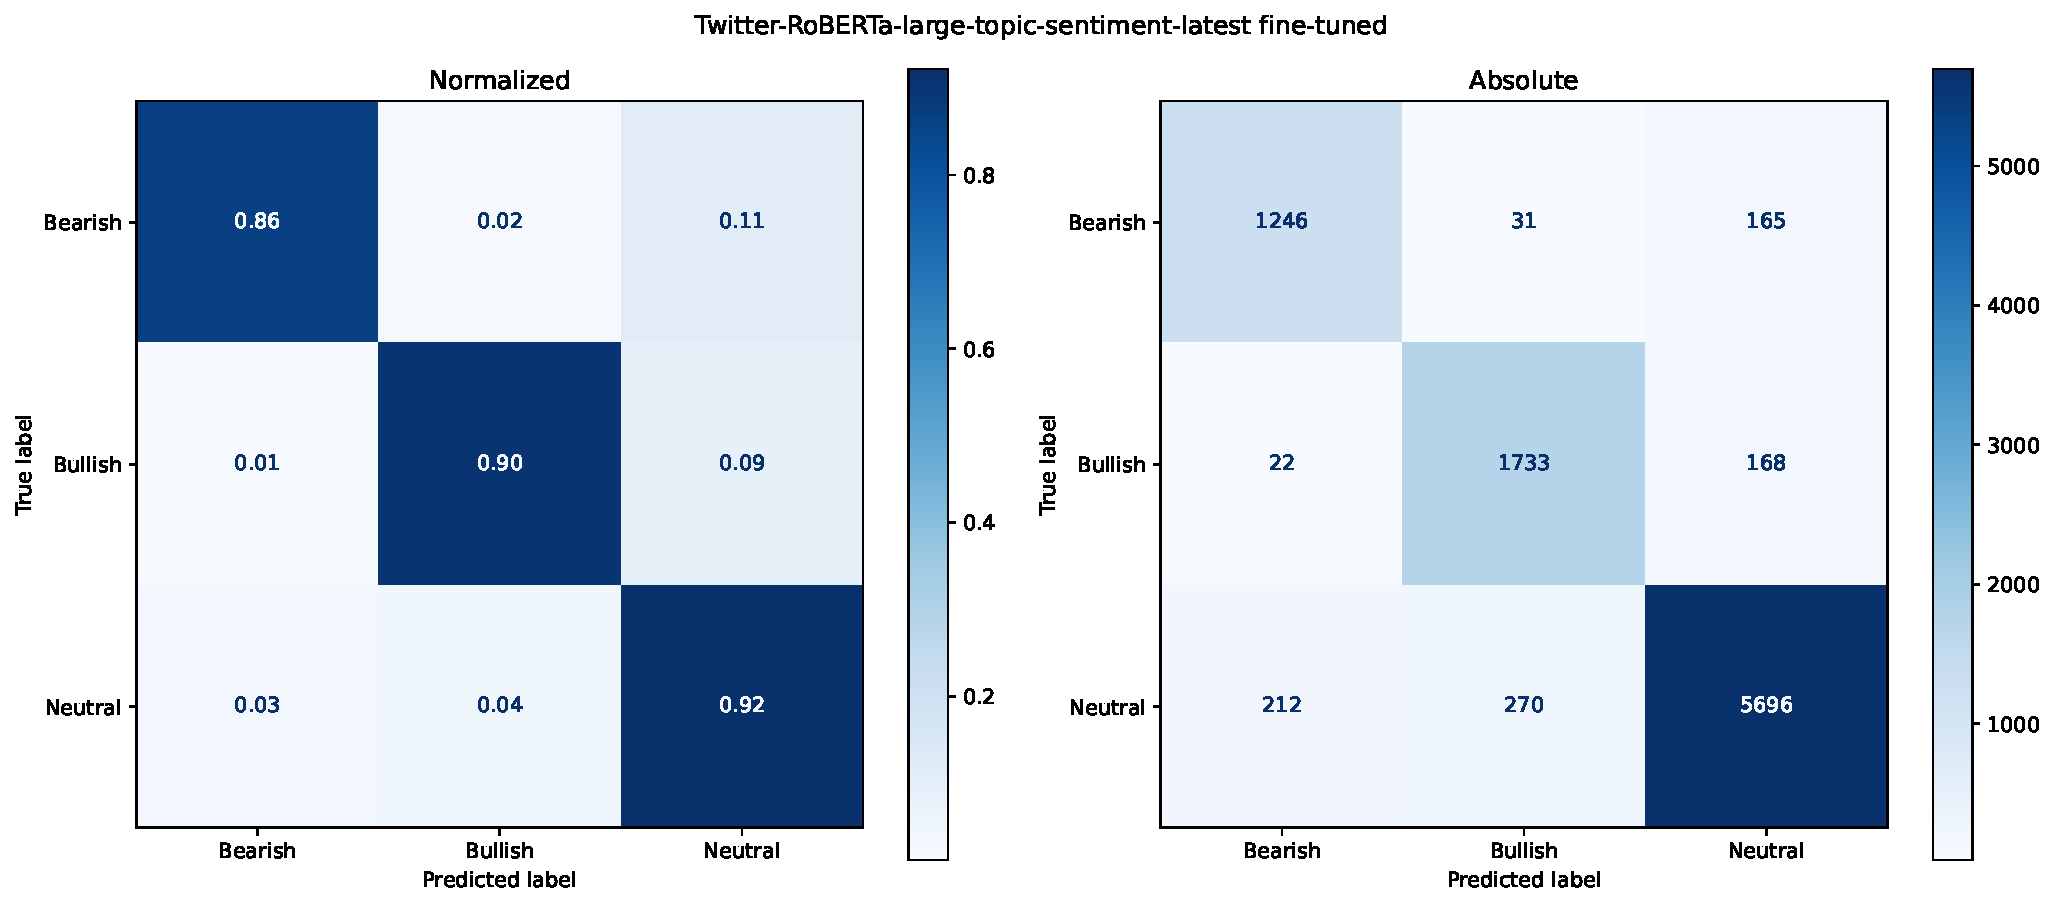
\includegraphics[width=0.96\linewidth]{confusion_matrix.pdf}
  \caption{Confusion matrix of the submitted fine-tuned Twitter--RoBERTa-large (normalised left,
  absolute counts right), from 5-fold out-of-fold predictions.}
  \label{fig:cm}
\end{figure}

Three qualitative failure modes remain: irony/sarcasm, mixed-signal tweets (`beats EPS but misses
revenue'), and domain jargon without explicit sentiment --- the ceiling for text-only models.

% ── 7. Agentic Workflow ──────────────────────────────────────────
\section{Extra Challenge 2 --- Agentic Workflow (+1.50 pts)}
We implement a conversational agent that orchestrates three classifiers with \emph{non-trivial},
adaptive routing. The implementation lives in \nolinkurl{src/agent.py} and
\nolinkurl{notebooks/08_Agentic_Workflow.ipynb}, and runs fully offline (a deterministic orchestrator
when no LLM key is present, plus an optional LangChain ReAct back-end; Yao et al., 2022).

\subsection{Architecture and Routing}
The agent exposes three tools --- \tH{VADER} (lexical baseline), \tH{LightGBM+SBERT} (ML model) and
\tH{FinBERT} (domain transformer) --- and routes adaptively:
\begin{itemize}
  \item VADER gives a quick lexical reading; if $|\text{compound}| > 0.3$ (strong signal) it is
  trusted directly.
  \item Otherwise LightGBM+SBERT is consulted; if it agrees with VADER, that is the verdict.
  \item On \emph{disagreement}, FinBERT is invoked as a domain-expert tie-breaker.
  \item The agent explains which model it trusted and why, and \texttt{ConversationBufferMemory}
  enables follow-up questions (``why did you classify that as Bearish?'').
\end{itemize}
This exceeds simple voting through signal-strength-based tool selection, explicit disagreement
detection with principled tie-breaking, and transparent reasoning. We validated the workflow
end-to-end: on a held-out sample it produces correct, explained verdicts (e.g.\ ``\$TSLA misses
estimates, downgrades'' $\to$ Bearish via FinBERT tie-break), and it is deterministic and
reproducible for the oral defence.

% ── 8. Conclusion ────────────────────────────────────────────────
\section{Conclusion}
This work delivers a complete NLP pipeline for financial tweet sentiment classification. Guided by a
Hugging Face backbone search, our \textbf{submitted single-model solution} --- an end-to-end
fine-tuned \textbf{Twitter--RoBERTa-large} --- achieves an out-of-fold macro-F1 of \textbf{0.8859},
a \textbf{+0.0838} gain over the 0.8021 baseline, and is also our best result overall, surpassing a
six-learner stacking ensemble (0.8483, extra work). Key contributions: (1) empirical evidence that
raw text beats preprocessing for financial tweets; (2) systematic evaluation of 11 feature
representations and 12 model families; (3) a transformer backbone search showing that a larger,
recent, domain-matched encoder is the decisive lever (and that DeBERTa-v3 needs fp32 yet still
trails); (4, extra) a fine-tuned GPT-2 \emph{decoder} classifier (0.7724) with the finding that
few-shot prompting of a small decoder collapses; (5, extra) a leakage-free stacking ensemble; and
(6, extra) an explainable, reproducible agentic workflow. Future work could explore domain-adaptive
pre-training on a larger financial-tweet corpus and multi-task learning with named-entity
recognition.

% ── References ───────────────────────────────────────────────────
\section*{References}
{\small
Akiba, T., Sano, S., Yanase, T., Ohta, T., \& Koyama, M. (2019). Optuna: A next-generation
hyperparameter optimization framework. \emph{KDD 2019}.

Alammar, J., \& Grootendorst, M. (2024). \emph{Hands-On Large Language Models: Language
Understanding and Generation}. O'Reilly Media. [Course textbook.]

Antweiler, W., \& Frank, M. Z. (2004). Is all that talk just noise? The information content of
internet stock message boards. \emph{Journal of Finance}, 59(3), 1259--1294.

Araci, D. (2019). FinBERT: Financial sentiment analysis with pre-trained language models.
\emph{arXiv:1908.10063}.

Barbieri, F., Camacho-Collados, J., Espinosa Anke, L., \& Neves, L. (2020). TweetEval: Unified
benchmark and comparative evaluation for tweet classification. \emph{EMNLP-Findings 2020}.

Bollen, J., Mao, H., \& Zeng, X. J. (2011). Twitter mood predicts the stock market. \emph{Journal of
Computational Science}, 2(1), 1--8.

Go, A., Bhayani, R., \& Huang, L. (2009). Twitter sentiment classification using distant
supervision. \emph{Stanford CS224N Report}.

He, P., Gao, J., \& Chen, W. (2021). DeBERTaV3: Improving DeBERTa using ELECTRA-style pre-training
with gradient-disentangled embedding sharing. \emph{arXiv:2111.09543}.

Hutto, C. J., \& Gilbert, E. (2014). VADER: A parsimonious rule-based model for sentiment analysis
of social media text. \emph{ICWSM 2014}.

Loureiro, D., Barbieri, F., Neves, L., Espinosa Anke, L., \& Camacho-Collados, J. (2022). TimeLMs:
Diachronic language models from Twitter. \emph{ACL 2022 (System Demonstrations); arXiv:2202.03829}.

Manning, C. D., Raghavan, P., \& Sch\"utze, H. (2008). \emph{Introduction to Information Retrieval}.
Cambridge University Press.

Mikolov, T., Chen, K., Corrado, G., \& Dean, J. (2013). Efficient estimation of word representations
in vector space. \emph{arXiv:1301.3781}.

Pennington, J., Socher, R., \& Manning, C. D. (2014). GloVe: Global vectors for word representation.
\emph{EMNLP 2014}.

Radford, A., Wu, J., Child, R., Luan, D., Amodei, D., \& Sutskever, I. (2019). Language models are
unsupervised multitask learners. \emph{OpenAI Blog}.

Reimers, N., \& Gurevych, I. (2019). Sentence-BERT: Sentence embeddings using Siamese BERT-networks.
\emph{EMNLP 2019}.

Rennie, J. D., Shih, L., Teevan, J., \& Karger, D. (2003). Tackling the poor assumptions of Naive
Bayes text classifiers. \emph{ICML 2003}.

Wolpert, D. H. (1992). Stacked generalization. \emph{Neural Networks}, 5(2), 241--259.

Yao, S., Zhao, J., Yu, D., Du, N., Shafran, I., Narasimhan, K., \& Cao, Y. (2022). ReAct:
Synergizing reasoning and acting in language models. \emph{arXiv:2210.03629}.

Zhao, T. Z., Wallace, E., Feng, S., Klein, D., \& Singh, S. (2021). Calibrate before use: Improving
few-shot performance of language models. \emph{ICML 2021}.
}

\end{document}
